\documentclass[10pt]{beamer}

\usetheme{metropolis}
\useoutertheme{metropolis}
\useinnertheme{metropolis}
\usefonttheme{metropolis}
%\usecolortheme{seahorse}   % or your preferred color theme
\usepackage{appendixnumberbeamer}
\usepackage{graphicx}
\usepackage{multirow}
\usepackage{booktabs}
\usepackage[scale=2]{ccicons}
\usepackage{xspace}
\usepackage[justification=centering]{caption}
\usepackage{braket}
\usepackage{amsmath}
\usepackage{verbatim}

\usepackage[version=3]{mhchem}
\definecolor{darkgreen}{RGB}{30, 133, 12}
\definecolor{lightgray}{gray}{0.9}
\renewcommand{\arraystretch}{1.2}

\title{Hartree-Fock Stability and its Relation to Strong Correlation}
% \subtitle{Applied to the Electron Gas}
\date{\today}
\author{Evan Curtin}
\institute{University of Illinois at Urbana-Champaign}
\titlegraphic{\hfill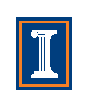
\includegraphics[height=1.5cm]{../figures/imark_bold.eps}}

\begin{document}

\maketitle

\begin{frame}{Table of contents}
  \setbeamertemplate{section in toc}[sections numbered]
  \tableofcontents[hideallsubsections]
\end{frame}

\section{Background Information}


\setbeamertemplate{frame footer}{
(Diradicals): Manabu Abe Chemical Reviews 2013 113 (9), 7011-7088 \newline
(Periodic): K.C. Rahnejat et al, Nature Comm. 2, 2011, 558
}
\begin{frame}{We Have Trouble Calculating...}
	\begin{columns}[c] % align columns
		\begin{column}{.5\textwidth}

	      \centering
		    	Polyradicals with degenerate triplet HOMO \\ \centering \vspace{5mm}
		    	\centering 
		    	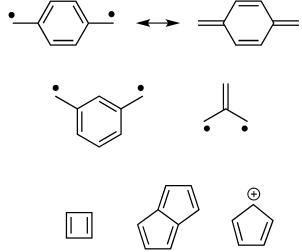
\includegraphics[width=0.8\linewidth]{../figures/diradicals.png}

		\end{column}
		\begin{column}{0.5\textwidth}		  
	      \centering
		    	Broken Symmetry Periodic Systems \\ \centering \vspace{5mm}
		    	\centering 
		    	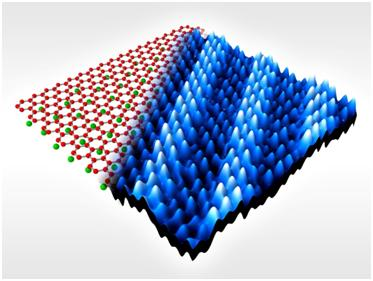
\includegraphics[width=0.8\linewidth]{../figures/CDW_Rahnejat.jpg}
		\end{column}
	\end{columns}
\end{frame}

\begin{frame}{The Electronic Structure Approach}
	\begin{itemize}[<+->]
		\item {The Molecular Electronic S.E. in the Born-Oppenheimer approximation
		  \begin{equation*}
  		  \left( 
        \hat{T}_{elec} + \hat{V}_{elec-nuc} 
                       + \hat{V}_{\textrm{\alert{elec-elec}}} 
  		 \right)
  		 \Psi
  		  = E_{exact}\Psi
		  \end{equation*}
		}
		\item {in Hartree-Fock theory is replaced by
		  \begin{equation*}
  		  \left( 
        \hat{T}_{elec} + \hat{V}_{elec-nuc} + 
  		   \hat{V}_{\textrm{\alert{mean-field}}} 
  		 \right)
  		 \Psi
  		  = E_{HF}\Psi
		  \end{equation*}
		}
		\item {the difference between the two energies is the \alert{correlation energy}
		  \begin{equation*}
		    E_{corr} = E_{exact} - E_{HF}
		  \end{equation*}
    }

	\end{itemize}
\end{frame}

\begin{frame}{Post-Hartree-Fock}
  \begin{itemize}
    \item {The correlation energy is recovered by post Hartree-Fock methods (CC, MBPT)
    which perform better the closer the HF solution is to the exact.} 
    \item {These methods may fail if the HF solution is far from the exact}
    \item {Can we remedy this by finding a better HF solution?}
  \end{itemize}
\end{frame}

{%+
\setbeamertemplate{frame footer}{}
\begin{frame}{Case Study: H$_2$ Dissociation}
  \centering
	Is this a lot of correlation or a bad reference?
	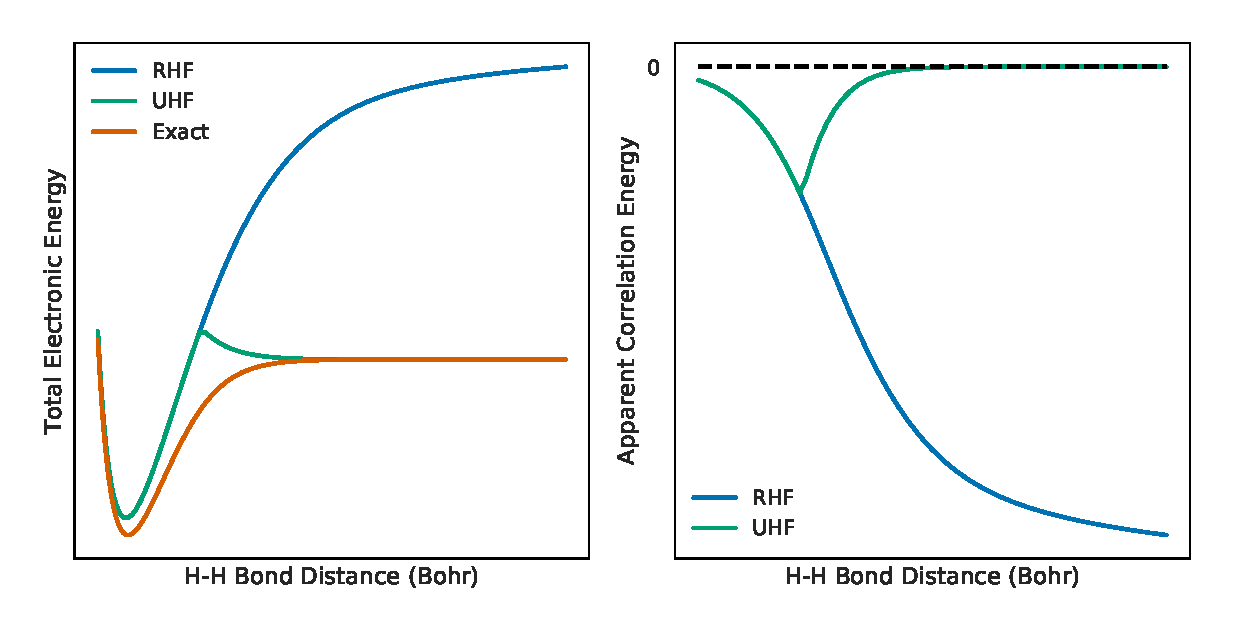
\includegraphics[width=\linewidth]{../figures/H2_curves.eps}
\end{frame}


{%
\setbeamertemplate{frame footer}{Seeger, R.; Pople, J. A. J. Chem. Phys. 1977, 66 (7), 3045.
}
\begin{frame}[fragile]{Hartree-Fock Theory is Almost Always Restricted}
	\begin{center}
		\begin{tabular}{ | c | c | c | c |}
			\hline
			 \textbf{Method} & \textbf{Spinorbital} & \textbf{DoF} & \textbf{Eigenfunction of}\\
			\hline
			Restricted \rule{0pt}{8ex} &
        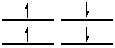
\includegraphics[width=0.2\linewidth]{../figures/rhf.jpg}
			& N/2
			& $\hat{S}^2$, $\hat{S}_z$
			\\ [4ex] \hline

			Unrestricted \rule{0pt}{8ex} &
			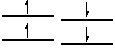
\includegraphics[width=0.2\linewidth]{../figures/uhf.jpg}
			& N & $\hat{S}_z$ \\ [4ex]
			\hline

			General \rule{0pt}{8ex} &
						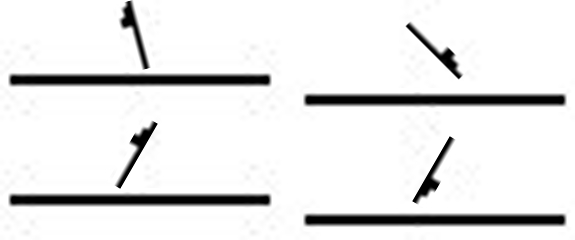
\includegraphics[width=0.2\linewidth]{../figures/ghf.jpg}
			& 2N & Neither \\ [4ex]
			\hline
		\end{tabular}
	\end{center}
\end{frame}

{%+
\setbeamertemplate{frame footer}{}
\begin{frame}{Case Study: H$_2$ Dissociation}
  \centering
	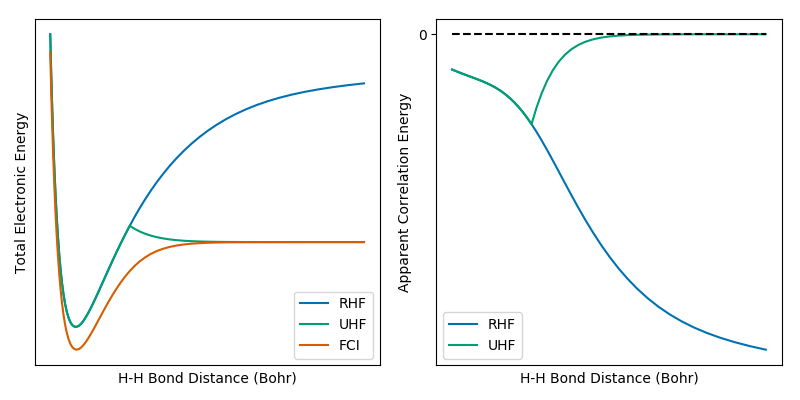
\includegraphics[width=\linewidth]{../figures/H2_curves.png}
	\begin{itemize}[<+->]
    \item {Is this situation unique to H$_2$ or is it common
    ?}
		\item {Can we identify when a better HF solution is necessary?}

	\end{itemize}
\end{frame}


\section{Hartree-Fock Stability}

{%
	\setbeamertemplate{frame footer}{Seeger, R.; Pople, J. A. J. Chem. Phys. 1977, 66 (7), 3045.}

\begin{frame}{Hartree-Fock Stability Conditions}
	\begin{itemize}[<+->]
		\item Solving the HF equations guarantees only that the energy is \alert{stationary}.
		\item{The solution is \alert{unstable} if any \alert{Orbital Hessian} (aka stability matrix, 
		electronic +
		Hessian) eigenvalues are \alert{negative}, indicating that it's not a minimum
			\begin{eqnarray}
				\begin{bmatrix}
					\bf{A}   & \bf{B}   \\
					\bf{B}^* & \bf{A}^* \\
				\end{bmatrix}
				\begin{bmatrix}  \bf{X} \\ \bf{Y}  \end{bmatrix}
				= \omega \begin{bmatrix}  \bf{X} \\ \bf{Y}  \end{bmatrix}
			\end{eqnarray}
		}
		\item{Where}
		\begin{eqnarray}
			A_{ia,jb} &=& \braket{{}_i^a|H-E_0|{}_j^b} = \left(\epsilon_a - \epsilon_i \right) \delta_{ij}\delta_{ab} + \braket{aj||ib}
			\nonumber \\
			B_{ia,jb} &=& \braket{{}_{ij}^{ab}|H-E_0|0} = \braket{ab||ij}.
		\end{eqnarray}
		\item{To determine instabilities, find the lowest eigenvalue}
	\end{itemize}
\end{frame}


{%
	\setbeamertemplate{frame footer}{1) Seeger, R.; Pople, J. A. J. Chem. Phys. 1977, 66 (7), 3045.}
\begin{frame}{Hartree-Fock Stability Conditions}
	\begin{itemize}
		\item[]{The Matrix Equation Factorizes} \\~\\
		\item[]{Singlet and Triplet Instabilities (RHF - RHF) and (RHF - UHF) }
	\end{itemize}
\end{frame}

\section{Homogeneous Electron Gas}

\begin{frame}
why

\end{frame}

{%
	\setbeamertemplate{frame footer}{Phillips, P. Advanced Solid State Physics, 2nd ed.; Cambridge University Press: Cambridge, 2012.}

\begin{frame}{Brief Overview of HEG}
	\begin{itemize}[<+->]
		\item{Homogeneous Electron Gas (HEG) model, also known as Uniform Electron Gas or Jellium 
		Model.}
		\item{Characterized by \alert{$r_s$}, inversely proportional to density}
		\item{Electrons in a box with "smeared" nuclei $\rightarrow$ uniform positive background charge}

		\item{The total charge is constrained to be neutral,}
			\begin{eqnarray}
				V_{bg}(\mathbf{r}) = \sum\limits_{i} \frac{-Ze^2}{|\mathbf{r}-\mathbf{R_i}|} \rightarrow -e^2 \int \frac{d\mathbf{r'}}{|\mathbf{r}-\mathbf{r'}|},
			\end{eqnarray}
		\item{and the background and coulomb terms cancel exactly,
			\begin{eqnarray}
				V_{ee} = e^2 \int \frac{d\mathbf{r'}}{|\mathbf{r}-\mathbf{r'}|}.
			\end{eqnarray}
		}
	\end{itemize}
\end{frame}

{%
	\setbeamertemplate{frame footer}{Giuliani, G.; Vignale, G. Quantum Theory of the Electron Liquid; 2005.}

\begin{frame}{Brief Overview of HEG}
	\begin{itemize}[<+->]
		\item{The discretized solutions are given by,
		\begin{eqnarray}\label{eq:hf_orb_energy}
			\epsilon_{\vec{k}}=
				\frac{\hbar^2 k^2}{2m} - \sum\limits_{\vec{k}'}^{|\vec{k}'|< k_f}
				\braket{\vec{k}, \vec{k}' |\vec{k}', \vec{k}}
		\end{eqnarray}
		}
		\item{Where the 2D and 3D two electron integral is given by
  		\begin{equation}
  			\braket{\vec{k}, \vec{k}'|\vec{k}'',\vec{k}'''}{=}
  				\begin{cases}
  				\frac{\pi}{V}\frac{2^{D-1}}{|\vec{k}-\vec{k}''|^{D-1}}
  				& \vec{k}''' = \vec{k}+\vec{k}'-\vec{k}'' \nonumber\\
  				0
  				& \text{else}
  				\end{cases}
  		\end{equation}
		}
		\item{ In 1D, if $V(r_{12}) = V_0\delta{(r_{12})}$,
		  \begin{equation}
  			\braket{k, k'|k'',k'''}{=}
  				\begin{cases}
  				V_0\text{ ;}
  				& k''' = k+k'-k'' \\
  				0\text{ ;}
  				& \text{else}
  				\end{cases}
		  \end{equation}
		}
	\end{itemize}
\end{frame}

{%
	\setbeamertemplate{frame footer}{Figure reproduced from: Ceperley, D. M.; Alder, B. J. Phys. Rev. 
	Lett. 1980, 45 (7), 
		566–569.}

\begin{frame}{Energies of Some Phases are Known Exactly}
  \centering
	QMC Energies for various phases
	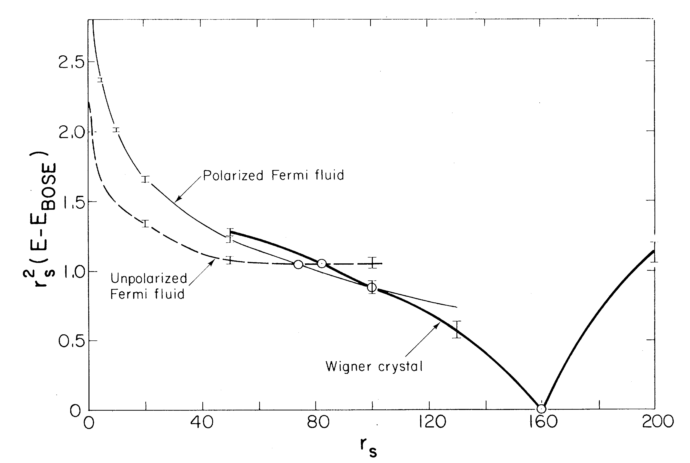
\includegraphics[width=.85\linewidth]{../figures/Ceperley_PhaseDiag.png}
\end{frame}


{%
\setbeamertemplate{frame footer}{Overhauser, A. W. Phys. Rev. Lett. 1960, 4 (9), 462–465.}
\begin{frame}{Applying HF-Stability to HEG}
	\begin{itemize}[<+->]
		\item{Will this predict the known tendency of crystallization at low density?}
		\item{Overhauser's theorem states that the GHF solution persists at all densities for the 
		HEG$^1$.}
		\begin{itemize}
  		\item{Can we show this numerically?}
  	\end{itemize}
	\end{itemize}
\end{frame}


\section{Implementation}

{%
\setbeamertemplate{frame footer}{}

\begin{frame}{Technical Challenges}
	\begin{columns}[c] % align columns
		\begin{column}{.4\textwidth}
			\begin{itemize}
			  \item {$\mathbf{H}$ Too big to construct or diagonalize}
				\item {Spectrum is dense, leading to numerical issues}
			\end{itemize}
		\end{column}
		\hfill
		\begin{column}{0.6\textwidth}
		    \begin{overprint}
			    \onslide<1>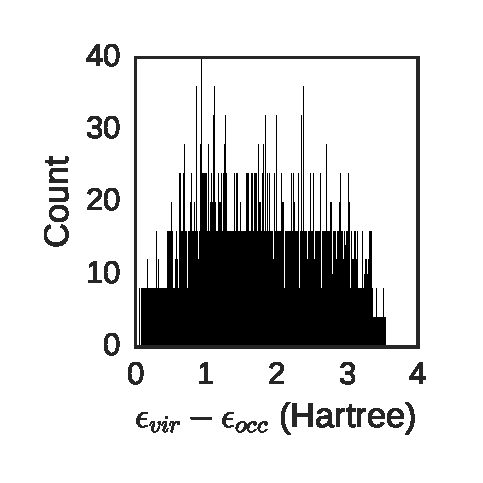
\includegraphics[width=\linewidth]{../figures/exchist.eps}
			\end{overprint}
		\end{column}
	\end{columns}
\end{frame}

{%
\setbeamertemplate{frame footer}{}

\begin{frame}{Implementation Solutions 1: Davidson's Algorithm}
	\begin{columns}[c] % align columns
		\begin{column}{.4\textwidth}
			\begin{itemize}
  			\item {Only need the lowest eigenvalue}
			  \item {Davidson requires no explicit matrix storage}
			  \item {Careful choice of initial guess circumvents numerical issues}
			  \item {Still slow for large N}
			\end{itemize}
		\end{column}
		\begin{column}{0.7\textwidth}
				\vspace{10mm}
		    \begin{overprint}
			    \onslide<1>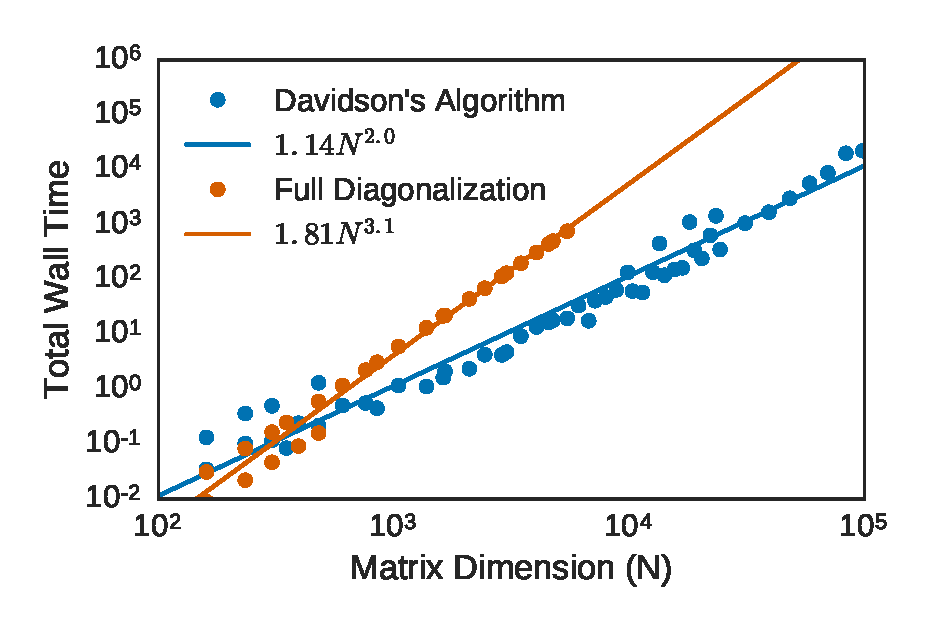
\includegraphics[width=\linewidth]{../figures/dav_vs_exact_scaling.eps}
			\end{overprint}
		\end{column}
	\end{columns}
\end{frame}

\begin{frame}{Implementation Solutions 2: Parallelization}
	\begin{columns}[c] % align columns
		\begin{column}{.4\textwidth}
			\begin{itemize}
			  \item {Enables utilization of Blue Waters}
			  \item {Depending on \# of cores, 400-1000 fold speedup compared to serial}			  			  
			  \item {This enabled me to compute 3D results}
			\end{itemize}
		\end{column}
		\begin{column}{0.7\textwidth}
		    \vspace{5mm}
		    \begin{overprint}
		    \centering
			    \onslide<1>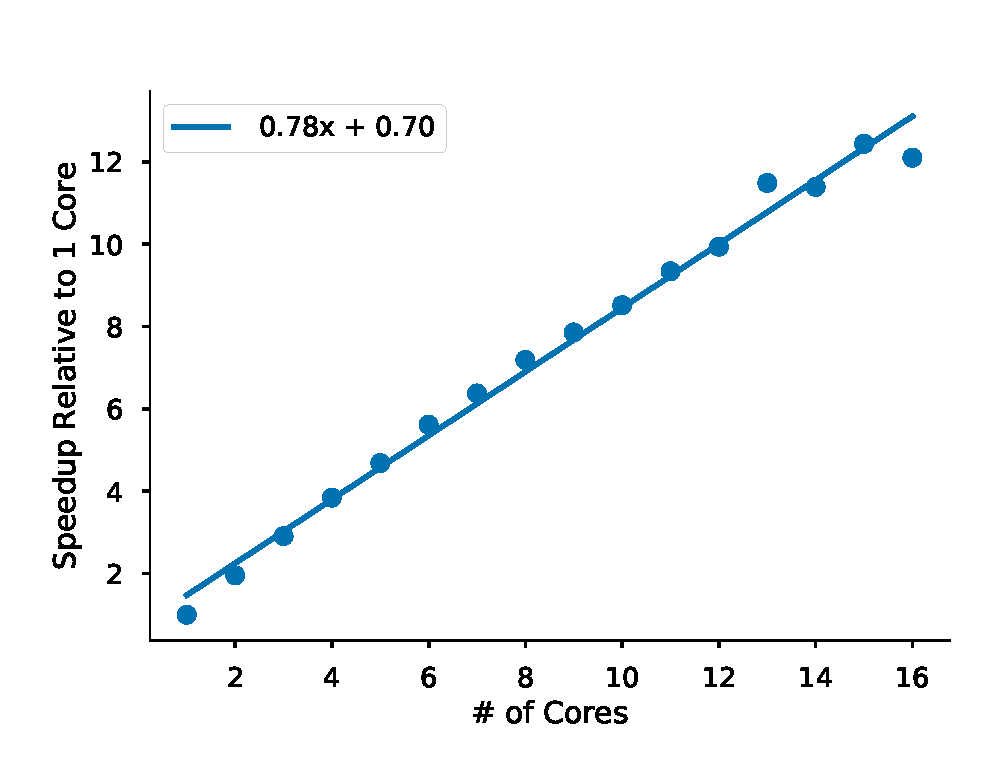
\includegraphics[width=0.9\linewidth]{../figures/parallel-scaling.eps}
			\end{overprint}
		\end{column}
	\end{columns}
\end{frame}

\section{Results}
{%
\setbeamertemplate{frame footer}{}
\begin{frame}{Stability Curves Show Clear Transition}
  \centering
  add each to own slide
	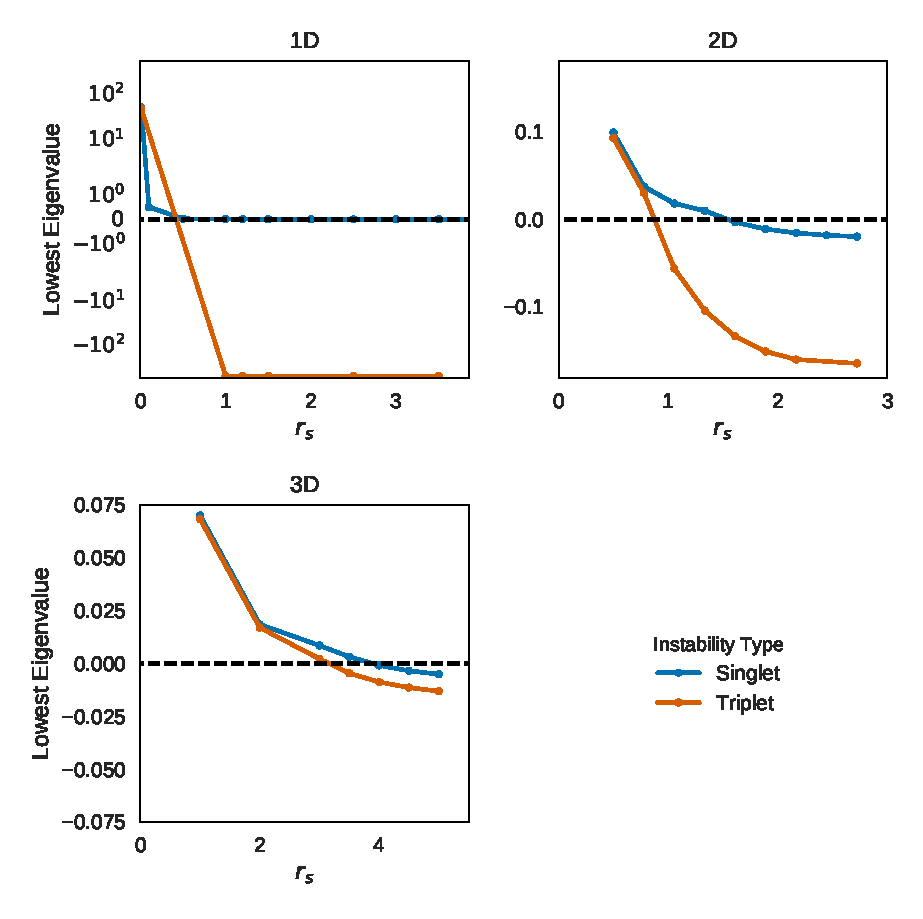
\includegraphics[width=0.75\linewidth]{../figures/stability.eps}
\end{frame}

\begin{frame}{Stability Onset Converges With k-points}
  \centering 
  \begin{overprint}
    \centering
    \onslide<1>\centering Singlet Instabilities\\ \vspace{5mm}
    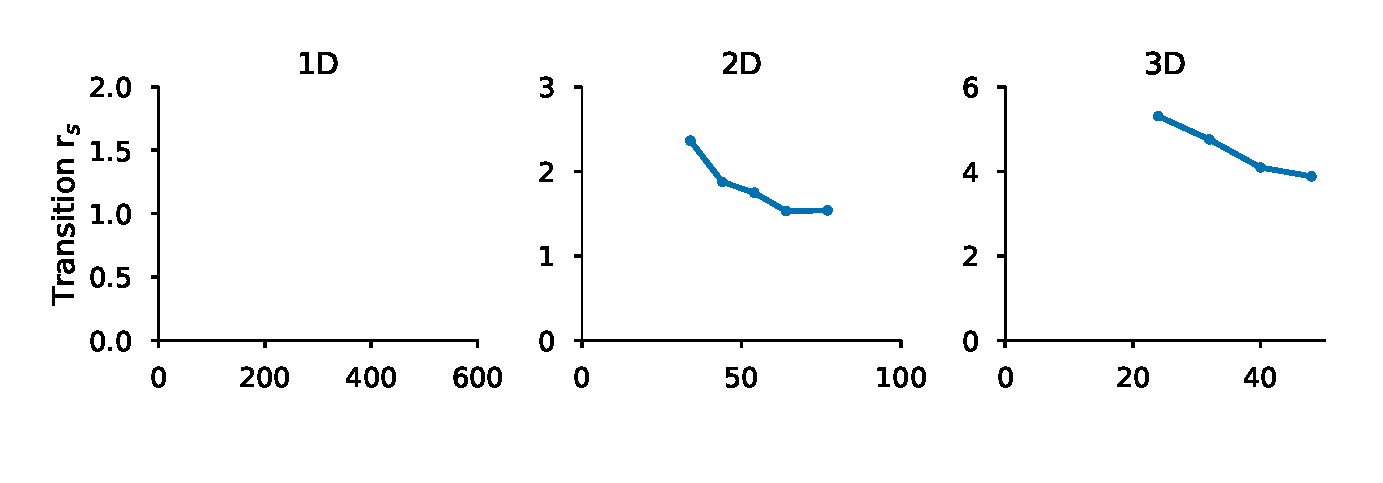
\includegraphics[width=\linewidth]{../figures/singlet_onset.eps}
  	\onslide<2>\centering Triplet Instabilities\\ \vspace{5mm}
  	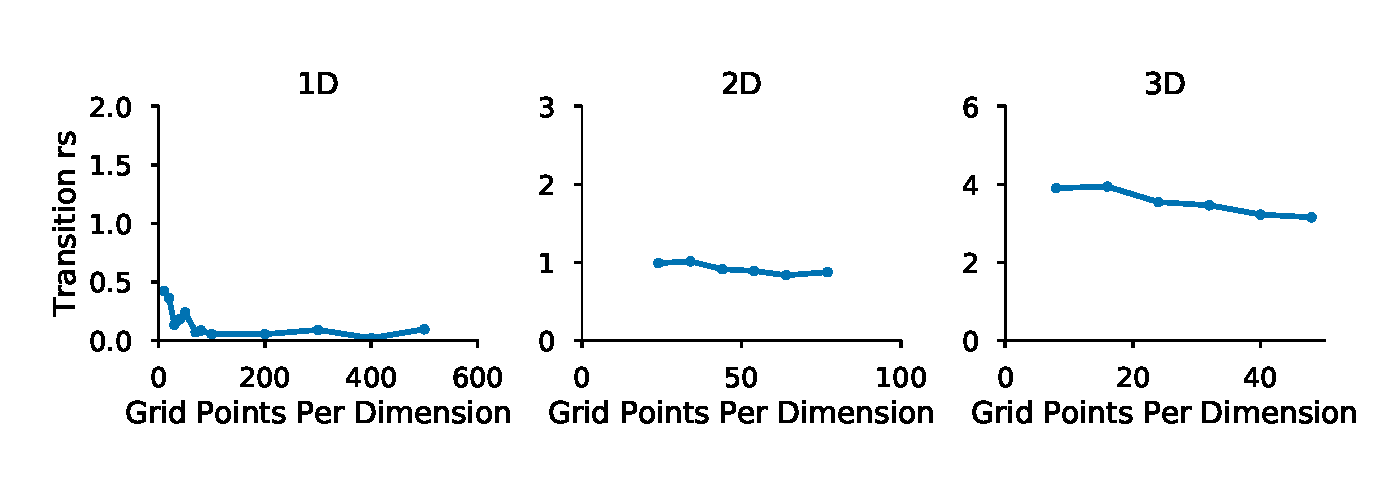
\includegraphics[width=\linewidth]{../figures/triplet_onset.eps}
	\end{overprint}
\end{frame}



{%
\setbeamertemplate{frame footer}{}
\begin{frame}{Transitions are Consistent with Others}
  \centering
  \begin{tabular}{ c | c | c } 
  \# Dimensions & Instability $r_s$ & Phase Boundary $r_s$ \\
  \hline
  1 & 0.(1) & 0$^1$ \\ 
  2 & 0.8(7)  & 0.8$^2$ \\ 
  3 & 3.(2)  & 3.0$^3$ \\ 
  \end{tabular}\\
  \vspace{5mm}
  \scriptsize
  (1) Overhauser, A. W. Phys. Rev. 1962, 128 (3), 1437–1452. \\
  (2) Bernu, B.; Delyon, F.; Holzmann, M.; Baguet, L. Phys. Rev. B 2011, 84 (11), 115115.\\
  (3) Baguet, L.; Delyon, F.; Bernu, B.; Holzmann, M. Phys. Rev. B 2014, 90 (16), 165131.
\end{frame}


\begin{frame}{Concluding Remarks}
  \begin{itemize}
    \item{ Paramagnetic HEG instabilities are successfully reproduced by the MO hessian approach }
    \item{ HF Stability analysis can show when restrictions should be lifted }
    \item{ It is feasible that even stable HF are not global minimum }
  \end{itemize}
\end{frame}

\section{Future Directions}

\setbeamertemplate{frame footer}{
(1) Ohno, K. Chem. Rec. 2016, 16 (5), 2198–2218. \newline
(2) Supady, A.; Blum, V.; Baldauf, C. J. Chem. Inf. Model. 2015, 55 (11), 2338–2348.
}
\begin{frame}{Brute Force GHF}
	\begin{itemize}[<+->]
  	\item Find the lowest energy GHF solution 
  	\item Use algorithms inspired by similar problems (atomic configuration)
  	\item Global Reaction Route Mapping (GRRM) / Anharmonic Downard Distortion (ADD)$^1$
  	\item Genetic Algorithm$^2$
	\end{itemize}
\end{frame}

\setbeamertemplate{frame footer}{
Figure reproduced from: Ohno, K. Chem. Rec. 2016, 16 (5), 2198–2218.
}
\begin{frame}{Anharmonic Downard Distortion}
  \centering
	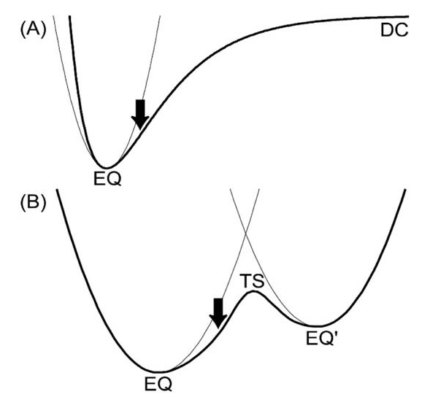
\includegraphics[width=.6\linewidth]{../figures/ADD.png}\\
	Replace atomic coordinates with MO coefficients and vibrational information with MO 
	eigenvalues/vectors
\end{frame}

\setbeamertemplate{frame footer}{
Figure reproduced from: Supady, A.; Blum, V.; Baldauf, C. J. Chem. Inf. Model. 2015, 55 (11), 
2338–2348.
}
\begin{frame}{Genetic Algorithm}
  \centering
  Genetic Algorithm promising in finding many low energy solutions
	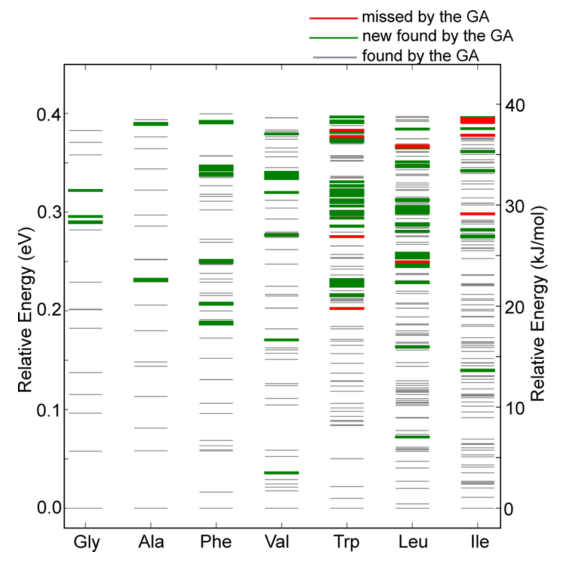
\includegraphics[width=.6\linewidth]{../figures/GA_supady.png}
\end{frame}

\setbeamertemplate{frame footer}{}
\begin{frame}{Proposal: Genetic Algorithm}
  \begin{itemize}
    \item{ Use as the gene the density matrix / MO coefficients }
    \item{ Less human input }
    \item{ Less dependence on underlying PES structure }
    \item{ How the HF solution gets found is irrelevant } 
  \end{itemize}
\end{frame}


\setbeamertemplate{frame footer}{}
\begin{frame}{Acknowledgements}
  \begin{itemize}
    \item{ Advisor: So Hirata }
    \item{ Group Members: 
      \begin{itemize}
        \item{ Misha Salim }
        \item{ Jacob Faucheaux }
        \item{ Alex Doran }
        \item{ Cole Johnson }
        \item{ Punit Jha }
        \item{ Alexander Kunitsa } 
        \item{ Jun Zhang } 
      \end{itemize}
    }
    \item{ Libraries: 
      \begin{itemize}
        \item{ PETSc }
        \item{ SLEPc }
      \end{itemize}
    }
    \item{ And the Blue Waters / NCSA Support Staff }
  \end{itemize}
\end{frame}


{%
\setbeamertemplate{frame footer}{}
\begin{frame}[standout]
  Questions?
\end{frame}


\appendix



{%
	\setbeamertemplate{frame footer}{Thouless, D. J. The Quantum Mechanics of Many-Body Systems, 2nd 
	ed.; Dover: 1972. (p. 114)}
\begin{frame}{Hartree-Fock Stability Derivation}
	\begin{itemize}[<+->]
		\item[]{The TDHF solution is given by the Liouville Von-Neumann Equation of Motion,
			\begin{eqnarray}
				i\hbar\frac{\partial \rho}{\partial t} = \left[ T+U, \rho \right],
			\end{eqnarray}
		}
		\item[]{Where U is the self-consistent potential,
			\begin{eqnarray}
				U_{pq} = \sum\limits_{p,q} \left(\rho_{pq,rs} - \braket{pr|sq} \right) \rho_{sr}.
			\end{eqnarray}
		}
		\item[]{Under the restrictions,
			\begin{eqnarray}
				\rho^2 = \rho \quad \textrm{and} \quad \rho^{\dagger} = \rho,
			\end{eqnarray}
		}
		\item[]{and to first order in $\rho_{ai}$, the elements of the density matrix are ,
			\begin{eqnarray}
				\rho_{ai} = C_{ai}, \quad \rho_{ia} = C_{ai}^*.
			\end{eqnarray}
		}
	\end{itemize}
\end{frame}

{%
	\setbeamertemplate{frame footer}{Thouless, D. J. The Quantum Mechanics of Many-Body Systems, 2nd 
	ed.; Dover: 1972. (p. 114)}

\begin{frame}{Hartree-Fock Stability Derivation}
	\begin{itemize}[<+->]
		\item[]{The TDHF EoM becomes,
			\begin{eqnarray}
				i\hbar \frac{dC_{ai} \left(t\right) }{dt} &=& \left(\epsilon_a - \epsilon_i \right) 
				\nonumber
					\\ &+& \sum\limits_{i}^{occ}  \sum\limits_{b}^{vir}
					  \left[\braket{aj||ib}C_{bj}   \left( t \right)
						  +\braket{ab||ij}C_{bj}^* \left( t \right) \right].
			\end{eqnarray}
		}
		\item[]{The solutions are complex exponentials,
			\begin{eqnarray}
				C_{ai} \left(t \right)  = \alpha X_{ai} e^{-i \omega t} + \alpha^* Y_{ai}^* e^{i \omega^* 
				t},
			\end{eqnarray}
		}
		\item[]{whose amplitudes, $X_{ai}$ and $Y_{ai}$ satisfy,
			\begin{align}
				\left(\epsilon_a - \epsilon_i \right)X_{ai} + \sum\limits_{i}^{occ}  \sum\limits_{b}^{vir}
					\left[ \braket{aj||ib}X_{bj} + \braket{ab||ij}Y_{bj} \right] &= \hbar \omega X_{ai}
				\nonumber \\
				\left(\epsilon_a - \epsilon_i \right)Y_{ai} + \sum\limits_{i}^{occ}  \sum\limits_{b}^{vir}
					\left[ \braket{aj||ib}X_{bj} + \braket{ab||ij}Y_{bj} \right] &= -\hbar \omega Y_{ai}.
			\end{align}
		}
		\item[]{These are the equations of the Random Phase Approximation (RPA)}
	\end{itemize}
\end{frame}


{%
 	\setbeamertemplate{frame footer}{}

\begin{frame}{Matrix Factorizations}
  \vspace{-6mm}
  \begin{eqnarray*}
    \begin{bmatrix}
      \mathbf{A} & \mathbf{B} \\
      \mathbf{B^*} & \mathbf{A^*} 
    \end{bmatrix}
    \begin{bmatrix}
      \mathbf{d} \\
      \mathbf{d^*} 
    \end{bmatrix}
    = 2E_2
    \begin{bmatrix}
      \mathbf{d} \\
      \mathbf{d^*} 
    \end{bmatrix}
  \end{eqnarray*}
  We can now apply the similarity transform defined by the Unitary matrix 
  \begin{eqnarray*}
    \mathbf{U} = \frac{1}{\sqrt{2}}
    \begin{bmatrix}
      \mathbf{I} & -\mathbf{I} \\
      \mathbf{I} & \mathbf{I} 
    \end{bmatrix}
  \end{eqnarray*}
  after which the transformed eigenvalue problem has the form
  \begin{eqnarray*}
    \frac{1}{2}
    \begin{bmatrix}
      \mathbf{A + B + A^* + B^*} & \mathbf{-A + A^* + B - B^*} \\
      \mathbf{-A + A^* - B + B^*} & \mathbf{A^* + A - B - B^*} 
    \end{bmatrix}
    \begin{bmatrix}
      \mathbf{d + d^*} \\
      \mathbf{d - d^*} 
    \end{bmatrix}
    &=& 2E_2
    \begin{bmatrix}
      \mathbf{d + d^*} \\
      \mathbf{-d + d^*} 
    \end{bmatrix} \\
    &=& 2E_2
    \begin{bmatrix}
      \mathbf{Re(d)} \\
      \mathbf{Im(d)} 
    \end{bmatrix}
  \end{eqnarray*}
  If $\mathbf{A}$ and $\mathbf{B}$ are both real, $\mathbf{A = A^*}$ and $\mathbf{B = B^*}$ and the 
  above simplifies to 
  \begin{eqnarray*}
    \begin{bmatrix}
      \mathbf{A + B} & \mathbf{0} \\
      \mathbf{0} & \mathbf{A - B} 
    \end{bmatrix}
    \begin{bmatrix}
      \mathbf{Re(d)} \\
      \mathbf{Im(d)} 
    \end{bmatrix}
    &=& 2E_2   
    \begin{bmatrix}
      \mathbf{Re(d)} \\
      \mathbf{Im(d)} 
    \end{bmatrix}
  \end{eqnarray*}
\end{frame}


\setbeamertemplate{frame footer}{
Figure reproduced from: Benavides-Riveros, C. L.; Lathiotakis, N. N.; Marques, M. A. L. 2017, 1–11.
}
\begin{frame}{Correlation Energy Increases at Small Gap}
  \centering
	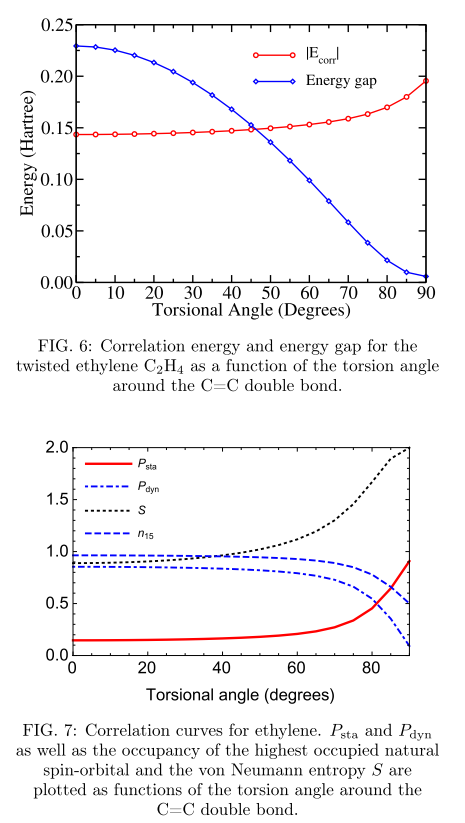
\includegraphics[width=.4\linewidth]{../figures/gap_vs_corr_Marques.png}
\end{frame}

\setbeamertemplate{frame footer}{
Phillips, P. Advanced Solid State Physics, 2nd ed.; Cambridge University Press: Cambridge, 2012.
}
\begin{frame}{Physicist's Strong Correlation}
  \centering
	\begin{quote}
  	However, because all repulsive short-range interactions renormalize towards the Fermi surface, 
  	their presence does not destroy the underlying free-particle picture of a Fermi Liquid. That 
  	is, the interactions can be integrated out, leaving behind renormalized electron or 
  	quasi-particle states. Hence, in a Fermi liquid there is a simple principle that can be invoked 
  	to lay plain that free electrons are the propagating degrees of freedom. Without the assumption 
  	of a Fermi surface, no principle exists that allows us to smooth away the interactions. 
  	\alert{We 
  	refer to such problems as being strongly correlated, namely those in which no obvious 
  	principle, ... exists that governs the renormalization of the electron-electron interactions.} 
	\end{quote}
	
\end{frame}

\section{Iterative Subspace Eigenvalue Methods}
{%
\setbeamertemplate{frame footer}{1. Saad, Y. Numerical Methods for Large Eigenvalue Problems; SIAM, 2011.

 2. Davidson, E. R. J. Comput. Phys. 1975, 17 (1), 87–94.}
\begin{frame}{Davidson's Algorithm}
  \begin{tabular}{l r}
    $\bf{Ax}=\lambda\bf{x}$         & Eigenvalue Problem \\
    $\bf{V}=[\bf{v_1,v_2,...,v_M}]$	& Guess vectors \\
    $\bf{\tilde{A}} = \bf{V}^\dag\bf{AV}$  & Transform into subspace\\ 
    $\bf{\tilde{A}\tilde{x}}=\tilde{\lambda}\bf{\tilde{x}}$ & Solve the subspace problem\\
  	$\mathbf{x_i} \approx \mathbf{x}_i^R = \mathbf{V\tilde{x}}_i$ & Approximate eigenvectors\\
  	$\lambda_i \approx \lambda_i^R = \tilde{\lambda}_i$ & Approximate eigenvalues \\
    $\mathbf{r}_i=\left(\mathbf{A}-\lambda_i\mathbf{I}\right)\mathbf{x}_i^R $ & Calculate the 
    residue \\
    $\mathbf{\delta}_i = c_i\mathbf{r}_i$ & Correction vectors \\
    $c_i = \frac{1}{\lambda_i\mathbf{I}-\mathbf{D}}$ & Diagonal Precondition \\
    $\mathbf{V} = 
    [\mathbf{v_1,v_2,...,v_M}\mathbf{,\delta}_1\mathbf{,\delta}_2,...\mathbf{,\delta}_l]$ & Append 
    to guess and restart \\ 
    $\mathbf{V} = orthonormalized(\mathbf{V})$ & Ensure orthonormal projection
  \end{tabular}
\end{frame}

{%
\setbeamertemplate{frame footer}{1. Saad, Y. Numerical Methods for Large Eigenvalue Problems; SIAM, 2011.

 2. Li, R.-C.; Zhang, L.-H. Convergence of Block Lanczos Method for Eigenvalue Clusters; 2013.}
\begin{frame}{Convergence Properties}
	\begin{itemize}[<+->]
		\item{The convergence of these subspace algorithms depends on:}
		\begin{itemize}
			\item{\alert{Number of eigenvalues} requested}
			\item{The \alert{block size} of the algorithm}
			\item{The \alert{density} of the eigenvalue spectrum}
			\item{The \alert{initial guess} eigenvectors}
			\item{The \alert{preconditioner} (Davidson only)}
		\end{itemize}
		\item{They can \alert{have convergence issues} if:}
		\begin{itemize}
			\item{The block size is too small compared to degeneracy}
			\item{The approximate eigenvectors become non-orthogonal}
		\end{itemize}
		\item{My recommendation for guess eigenvectors is
		\begin{eqnarray}
			v_j^{(i)} = normalize\left(\frac{1}{|A_{ii} - A_{jj}| + 1} \right).
		\end{eqnarray}
		}
	\end{itemize}
\end{frame}




{%
\setbeamertemplate{frame footer}{Hern, V.; Tom, A.; Vidal, V. SLEPc Technical Reports, 2007.}
\begin{frame}{Orthogonalization}
	\begin{itemize}
		\item{The condition number, $\kappa$, is bound from below by
			\begin{eqnarray}
				\kappa \geq \frac{Max(A_{ii})}{Min(A_{jj})}
			\end{eqnarray}
		}
		\item{The Gram-Schmidt procedure has numerical issues,
			\begin{eqnarray}
				||\mathbf{I} - \mathbf{Q^TQ}|| \leq \frac{\alpha\kappa^2}{1-\beta\kappa^2}.
			\end{eqnarray}
		}
		\item{Modified Gram-Schmidt is better, but not perfect,
			\begin{eqnarray}
				||\mathbf{I} - \mathbf{Q^TQ}|| \leq \frac{\gamma\kappa}{1-\eta\kappa}
			\end{eqnarray}
		}
		\item{May need multiple orthogonalization steps}
	\end{itemize}

\end{frame}


%\begin{frame}
%		{
%			\resizebox{0.9\textwidth}{!}{%
%			\begin{tabular}{r@{\qquad}cccccc}
%				  \multirow{1}{*}{Solution Type} & \multicolumn{6}{c}{Space Type}  \\
%				  \cmidrule{2-7}
%%				  \midrule
%				  Real RHF    & ${}^1\mathbf{A}' + {}^1\mathbf{B}'$ & ${}^1\mathbf{A}' - {}^1\mathbf{B}'$ & 
%				  ${}^3\mathbf{A}' + {}^3\mathbf{B}'$ & ${}^3\mathbf{A}' - {}^3\mathbf{B}'$ & 
%				  ${}^3\mathbf{A}' + {}^3\mathbf{B}'$ & ${}^3\mathbf{A}' - {}^3\mathbf{B}'$  \\
%				  Complex RHF & - & \alert{${}^1\mathbf{H}'$} & - & \alert{${}^3\mathbf{H}'$} & - & 
%				  ${}^3\mathbf{H}'$ \\
%				  Real UHF    & - & - & $\mathbf{A}' + \mathbf{B}'$ & $\mathbf{A}' - \mathbf{B}'$ & 
%				  $\mathbf{A}'' + \mathbf{B}''$ & $\mathbf{A}'' - \mathbf{B}''$ \\
%				  Complex UHF & - & - & - &  $\mathbf{H}'$ & - & $\mathbf{H}'$ \\
%				  Real GHF    & - & - & - & - & $\mathbf{A} - \mathbf{B}$ &  $\mathbf{A} - \mathbf{B}$  \\
%				  Complex GHF & - & - & - & - & - & $\mathbf{H}$ \\
%				  \bottomrule
%			\end{tabular}}
%
%		}
%\end{frame}

\end{document}
